\documentclass{article}
\usepackage{graphics} 
\usepackage{hyperref}

\author{Kevin Zollicoffer}
\title{Predictive Modeling\\Lesson 3\\\emph{Logistical Regression and Neural Networks}}
\date{09/29/2013}

\usepackage{Sweave}
\begin{document}
\maketitle
%\tableofcontents
\Sconcordance{concordance:NeuralNetworks.tex:NeuralNetworks.Rnw:%
1 8 1 1 0 15 1 1 2 1 0 1 1 40 0 1 2 2 1 1 2 1 0 5 1 3 0 1 2 2 1 1 2 1 0 %
3 1 3 0 1 2 3 1 1 2 1 0 1 2 39 0 1 2 73 0 1 2 49 0 1 2 208 0 1 3 2 1 1 %
2 1 0 1 1 7 0 1 2 2 1 1 2 1 0 2 1 36 0 1 2 1 1 1 2 1 0 3 1 3 0 1 2 3 1 %
1 2 1 0 1 1 3 0 1 2 2 1 1 9 7 0 1 6 4 0 2 1 401 0 1 2 3 1 1 2 1 0 1 1 %
13 0 1 2 8 0 1 2 233 0 1 2 2 1 1 2 1 0 1 1 12 0 1 2 1 1 1 2 1 0 3 1 3 0 %
1 2 3 1 1 2 1 0 1 1 3 0 1 2 30 1}


\section*{Introduction}
I chose to use R for the assignments. This is my first class in the PASS program and one of my goals upon completion of PASS is to be proficient in R. 
\\
\\
\noindent
The RStudio project files and accompanying artifacts, including the tex file that created this PDF, are publicly available on GitHub
\\
\url{https://github.com/zollie/PASS-PredictiveModeling-LogisticalRegression}

\section*{Data Setup}
I took the Excel spreadsheet and saved it as a CSV for easy import into R
\begin{Schunk}
\begin{Sinput}
> gc <- read.csv("~/R/PASS/PredictiveModeling/LogisticRegression/GermanCredit.csv")
> head(gc)
\end{Sinput}
\begin{Soutput}
  OBS. CHK_ACCT DURATION HISTORY NEW_CAR USED_CAR FURNITURE RADIO.TV EDUCATION
1    1        0        6       4       0        0         0        1         0
2    2        1       48       2       0        0         0        1         0
3    3        3       12       4       0        0         0        0         1
4    4        0       42       2       0        0         1        0         0
5    5        0       24       3       1        0         0        0         0
6    6        3       36       2       0        0         0        0         1
  RETRAINING AMOUNT SAV_ACCT EMPLOYMENT INSTALL_RATE MALE_DIV MALE_SINGLE
1          0   1169        4          4            4        0           1
2          0   5951        0          2            2        0           0
3          0   2096        0          3            2        0           1
4          0   7882        0          3            2        0           1
5          0   4870        0          2            3        0           1
6          0   9055        4          2            2        0           1
  MALE_MAR_or_WID CO.APPLICANT GUARANTOR PRESENT_RESIDENT REAL_ESTATE
1               0            0         0                4           1
2               0            0         0                2           1
3               0            0         0                3           1
4               0            0         1                4           0
5               0            0         0                4           0
6               0            0         0                4           0
  PROP_UNKN_NONE AGE OTHER_INSTALL RENT OWN_RES NUM_CREDITS JOB NUM_DEPENDENTS
1              0  67             0    0       1           2   2              1
2              0  22             0    0       1           1   2              1
3              0  49             0    0       1           1   1              2
4              0  45             0    0       0           1   2              2
5              1  53             0    0       0           2   2              2
6              1  35             0    0       0           1   1              2
  TELEPHONE FOREIGN RESPONSE
1         1       0        1
2         0       0        0
3         0       0        1
4         0       0        1
5         0       0        0
6         1       0        1
\end{Soutput}
\end{Schunk}

\noindent
The categorical predictors are turned into factors for R
\begin{Schunk}
\begin{Sinput}
> gc$RESPONSE <- factor(gc$RESPONSE)
> gc$JOB <- factor(gc$JOB)
> gc$EMPLOYMENT <- factor(gc$EMPLOYMENT)
> gc$SAV_ACCT <- factor(gc$SAV_ACCT)
> gc$HISTORY <- factor(gc$HISTORY)
> gc$CHK_ACCT <- factor(gc$CHK_ACCT)
\end{Sinput}
\end{Schunk}

\section*{Partitioning}
Next, the data is paritioned into 60\% Train and 40\% Test sets. I set the RNG seed for reproducibility
\begin{Schunk}
\begin{Sinput}
> n <- nrow(gc)
> a <- sort(sample(1:n, floor(n*.6)))
> gc.train <- gc[a,]
> gc.test <- gc[-a,]
\end{Sinput}
\end{Schunk}

\section*{Logistical Regression}
A Logistical Regression model is fit to the train data. 

\begin{Schunk}
\begin{Sinput}
> logit <- glm(RESPONSE ~ CHK_ACCT+DURATION+HISTORY+NEW_CAR+USED_CAR+FURNITURE+RADIO.TV+EDUCATION+RETRAINING+AMOUNT+SAV_ACCT+EMPLOYMENT+INSTALL_RATE+MALE_DIV+MALE_SINGLE+MALE_MAR_or_WID+CO.APPLICANT+GUARANTOR+PRESENT_RESIDENT+REAL_ESTATE+PROP_UNKN_NONE+AGE+OTHER_INSTALL+RENT+OWN_RES+NUM_CREDITS+JOB+NUM_DEPENDENTS+TELEPHONE+FOREIGN, data=gc.train, family=binomial("logit"))
> logit
\end{Sinput}
\begin{Soutput}
Call:  glm(formula = RESPONSE ~ CHK_ACCT + DURATION + HISTORY + NEW_CAR + 
    USED_CAR + FURNITURE + RADIO.TV + EDUCATION + RETRAINING + 
    AMOUNT + SAV_ACCT + EMPLOYMENT + INSTALL_RATE + MALE_DIV + 
    MALE_SINGLE + MALE_MAR_or_WID + CO.APPLICANT + GUARANTOR + 
    PRESENT_RESIDENT + REAL_ESTATE + PROP_UNKN_NONE + AGE + OTHER_INSTALL + 
    RENT + OWN_RES + NUM_CREDITS + JOB + NUM_DEPENDENTS + TELEPHONE + 
    FOREIGN, family = binomial("logit"), data = gc.train)

Coefficients:
     (Intercept)         CHK_ACCT1         CHK_ACCT2         CHK_ACCT3  
       1.9382673         0.5023131         1.3497380         1.9452021  
        DURATION          HISTORY1          HISTORY2          HISTORY3  
      -0.0276555        -0.2593253         0.3418115         0.5251609  
        HISTORY4           NEW_CAR          USED_CAR         FURNITURE  
       1.4275518        -0.6117829         0.3965193         0.1576746  
        RADIO.TV         EDUCATION        RETRAINING            AMOUNT  
       0.4949101        -0.1705930        -0.0767318        -0.0001219  
       SAV_ACCT1         SAV_ACCT2         SAV_ACCT3         SAV_ACCT4  
       0.8681562         0.7210853         1.1493753         1.2641500  
     EMPLOYMENT1       EMPLOYMENT2       EMPLOYMENT3       EMPLOYMENT4  
       0.1620601         0.4523329         1.3759836         0.6672299  
    INSTALL_RATE          MALE_DIV       MALE_SINGLE   MALE_MAR_or_WID  
      -0.3684956        -0.3868091         0.4472375         0.2917269  
    CO.APPLICANT         GUARANTOR  PRESENT_RESIDENT       REAL_ESTATE  
      -0.6288904         1.1317737        -0.1494562         0.0599302  
  PROP_UNKN_NONE               AGE     OTHER_INSTALL              RENT  
      -0.8477059         0.0153764        -0.6176907        -0.7773178  
         OWN_RES       NUM_CREDITS              JOB1              JOB2  
      -0.5930748        -0.1931763        -0.4742573        -0.7608312  
            JOB3    NUM_DEPENDENTS         TELEPHONE           FOREIGN  
      -0.3479994        -0.2218640         0.5463572         2.8128361  

Degrees of Freedom: 599 Total (i.e. Null);  556 Residual
Null Deviance:	    738 
Residual Deviance: 516.1 	AIC: 604.1
\end{Soutput}
\begin{Sinput}
> summary(logit)
\end{Sinput}
\begin{Soutput}
Call:
glm(formula = RESPONSE ~ CHK_ACCT + DURATION + HISTORY + NEW_CAR + 
    USED_CAR + FURNITURE + RADIO.TV + EDUCATION + RETRAINING + 
    AMOUNT + SAV_ACCT + EMPLOYMENT + INSTALL_RATE + MALE_DIV + 
    MALE_SINGLE + MALE_MAR_or_WID + CO.APPLICANT + GUARANTOR + 
    PRESENT_RESIDENT + REAL_ESTATE + PROP_UNKN_NONE + AGE + OTHER_INSTALL + 
    RENT + OWN_RES + NUM_CREDITS + JOB + NUM_DEPENDENTS + TELEPHONE + 
    FOREIGN, family = binomial("logit"), data = gc.train)

Deviance Residuals: 
    Min       1Q   Median       3Q      Max  
-2.6286  -0.6632   0.3267   0.6882   2.3683  

Coefficients:
                   Estimate Std. Error z value Pr(>|z|)    
(Intercept)       1.9382673  1.4776338   1.312 0.189609    
CHK_ACCT1         0.5023131  0.2868664   1.751 0.079940 .  
CHK_ACCT2         1.3497380  0.4836687   2.791 0.005261 ** 
CHK_ACCT3         1.9452021  0.3192069   6.094  1.1e-09 ***
DURATION         -0.0276555  0.0124606  -2.219 0.026457 *  
HISTORY1         -0.2593253  0.7520851  -0.345 0.730238    
HISTORY2          0.3418115  0.5779081   0.591 0.554210    
HISTORY3          0.5251609  0.6465567   0.812 0.416652    
HISTORY4          1.4275518  0.6074964   2.350 0.018779 *  
NEW_CAR          -0.6117829  0.4710751  -1.299 0.194049    
USED_CAR          0.3965193  0.5901390   0.672 0.501642    
FURNITURE         0.1576746  0.4957144   0.318 0.750428    
RADIO.TV          0.4949101  0.4771533   1.037 0.299636    
EDUCATION        -0.1705930  0.6203380  -0.275 0.783316    
RETRAINING       -0.0767318  0.5454558  -0.141 0.888127    
AMOUNT           -0.0001219  0.0000594  -2.053 0.040091 *  
SAV_ACCT1         0.8681562  0.3898857   2.227 0.025968 *  
SAV_ACCT2         0.7210853  0.5510039   1.309 0.190644    
SAV_ACCT3         1.1493753  0.6084248   1.889 0.058878 .  
SAV_ACCT4         1.2641500  0.3468265   3.645 0.000267 ***
EMPLOYMENT1       0.1620601  0.6197901   0.261 0.793726    
EMPLOYMENT2       0.4523329  0.5973562   0.757 0.448915    
EMPLOYMENT3       1.3759836  0.6467280   2.128 0.033370 *  
EMPLOYMENT4       0.6672299  0.5917302   1.128 0.259492    
INSTALL_RATE     -0.3684956  0.1254429  -2.938 0.003308 ** 
MALE_DIV         -0.3868091  0.5679873  -0.681 0.495861    
MALE_SINGLE       0.4472375  0.2796380   1.599 0.109744    
MALE_MAR_or_WID   0.2917269  0.4283643   0.681 0.495855    
CO.APPLICANT     -0.6288904  0.5098314  -1.234 0.217379    
GUARANTOR         1.1317737  0.5825667   1.943 0.052048 .  
PRESENT_RESIDENT -0.1494562  0.1192233  -1.254 0.209994    
REAL_ESTATE       0.0599302  0.2879804   0.208 0.835147    
PROP_UNKN_NONE   -0.8477059  0.5776286  -1.468 0.142223    
AGE               0.0153764  0.0119257   1.289 0.197275    
OTHER_INSTALL    -0.6176907  0.2814590  -2.195 0.028192 *  
RENT             -0.7773178  0.6646814  -1.169 0.242219    
OWN_RES          -0.5930749  0.6382663  -0.929 0.352787    
NUM_CREDITS      -0.1931763  0.2533597  -0.762 0.445786    
JOB1             -0.4742573  0.8666457  -0.547 0.584219    
JOB2             -0.7608312  0.8284276  -0.918 0.358407    
JOB3             -0.3479994  0.8215027  -0.424 0.671848    
NUM_DEPENDENTS   -0.2218640  0.3296838  -0.673 0.500973    
TELEPHONE         0.5463572  0.2722419   2.007 0.044762 *  
FOREIGN           2.8128361  1.1654728   2.413 0.015801 *  
---
Signif. codes:  0 ‘***’ 0.001 ‘**’ 0.01 ‘*’ 0.05 ‘.’ 0.1 ‘ ’ 1

(Dispersion parameter for binomial family taken to be 1)

    Null deviance: 738.05  on 599  degrees of freedom
Residual deviance: 516.08  on 556  degrees of freedom
AIC: 604.08

Number of Fisher Scoring iterations: 6
\end{Soutput}
\begin{Sinput}
> confint(logit)
\end{Sinput}
\begin{Soutput}
                         2.5 %        97.5 %
(Intercept)      -0.9483086330  4.863639e+00
CHK_ACCT1        -0.0578207835  1.068824e+00
CHK_ACCT2         0.4378136712  2.350091e+00
CHK_ACCT3         1.3330469901  2.587685e+00
DURATION         -0.0522896603 -3.314751e-03
HISTORY1         -1.7402640699  1.223633e+00
HISTORY2         -0.7808915320  1.504650e+00
HISTORY3         -0.7256874803  1.825148e+00
HISTORY4          0.2565070787  2.656288e+00
NEW_CAR          -1.5571580335  2.974326e-01
USED_CAR         -0.7578591898  1.565918e+00
FURNITURE        -0.8287903738  1.122608e+00
RADIO.TV         -0.4569724061  1.422208e+00
EDUCATION        -1.3959785104  1.045972e+00
RETRAINING       -1.1572272270  9.894845e-01
AMOUNT           -0.0002399121 -6.296406e-06
SAV_ACCT1         0.1201717191  1.653509e+00
SAV_ACCT2        -0.2962365829  1.891110e+00
SAV_ACCT3         0.0224850597  2.440544e+00
SAV_ACCT4         0.6034520555  1.967469e+00
EMPLOYMENT1      -1.0576078319  1.383995e+00
EMPLOYMENT2      -0.7198677682  1.633857e+00
EMPLOYMENT3       0.1169650710  2.664044e+00
EMPLOYMENT4      -0.4959761843  1.834425e+00
INSTALL_RATE     -0.6188734195 -1.261201e-01
MALE_DIV         -1.4930941050  7.473492e-01
MALE_SINGLE      -0.1006843166  9.977084e-01
MALE_MAR_or_WID  -0.5325003697  1.155354e+00
CO.APPLICANT     -1.6384002108  3.774832e-01
GUARANTOR         0.0533049350  2.374182e+00
PRESENT_RESIDENT -0.3847713927  8.363036e-02
REAL_ESTATE      -0.5023666600  6.291340e-01
PROP_UNKN_NONE   -1.9879964697  2.860277e-01
AGE              -0.0077129936  3.914491e-02
OTHER_INSTALL    -1.1706848175 -6.451552e-02
RENT             -2.0954129284  5.165607e-01
OWN_RES          -1.8648210754  6.464762e-01
NUM_CREDITS      -0.6927616526  3.028382e-01
JOB1             -2.1958101803  1.234842e+00
JOB2             -2.4111794352  8.720063e-01
JOB3             -1.9856813573  1.268323e+00
NUM_DEPENDENTS   -0.8654599921  4.310456e-01
TELEPHONE         0.0180926715  1.087650e+00
FOREIGN           0.9137954618  5.869858e+00
\end{Soutput}
\begin{Sinput}
> residuals(logit)
\end{Sinput}
\begin{Soutput}
          3           7           8           9          11          12 
 0.16418010  0.38743896  0.88183793  0.16138331 -0.79806588 -0.34783101 
         14          17          18          21          23          26 
-1.27817393  0.18993479  1.91211963  0.47009851  0.24084261  0.66508158 
         27          28          29          30          31          33 
 0.46612077  0.56632233  0.45196101 -0.50626160  0.86255313  0.88515134 
         34          35          36          37          38          39 
 0.25407197  0.82795004 -1.21375613  0.62542921 -1.22484012  0.41397534 
         40          41          42          43          44          45 
 0.93169606  0.46806015  0.63093058  0.84193263  0.51087077 -0.67149662 
         47          51          55          57          58          59 
 0.49474831  0.92723575 -0.69986926 -2.11506595  0.80617703  0.95772000 
         61          62          63          64          65          66 
 0.86888228  0.14056573 -1.19715252 -0.58020034  0.81347650  0.53626890 
         67          68          69          70          71          72 
 0.69149104  0.92964847 -1.23700996  0.58120364  0.97603122  0.08928786 
         73          74          75          77          78          79 
 0.75778204  0.86492679 -1.23621285 -0.65529291  0.48560410  0.59023426 
         82          84          86          88          89          91 
 0.31894771  0.74325594  0.18638107 -1.13665340  0.75973216  0.23294774 
         92          94          96          97          98         100 
 0.61423719  0.87604452 -0.24028419  0.14146960  1.03768538  0.53804572 
        101         102         103         106         108         109 
 0.62053161  1.10790167  0.43053256 -1.26732506  0.93236258  0.22733145 
        110         111         112         113         114         115 
 0.39063804  0.89703985  1.16314516  1.17626016 -1.10867082  0.63683688 
        116         118         119         120         121         122 
 0.15956435  0.21663286 -1.47975769  0.39036034 -1.19742448  0.32575020 
        123         125         126         127         128         131 
 0.48225038 -1.27801048  1.26805930  0.96544487 -1.25979820  1.02044056 
        134         135         136         137         138         139 
 1.02914582  0.52959194  0.13391115  0.40215164 -2.12305620  0.15365805 
        140         141         143         145         146         149 
 0.39035052  0.08537530  1.10778951  0.54541784  1.19740625  0.80234167 
        151         153         155         156         157         158 
 0.26043147  1.05608187  0.61907344 -0.94353693  0.07784126  1.51549140 
        159         160         161         162         163         164 
 0.74644018  0.08634070  0.16911524  0.75458797  0.25418888  1.39146749 
        165         166         169         171         175         176 
 0.77286307  0.18342711  0.44690093 -0.53470996 -0.95686950 -1.78526898 
        179         181         182         184         185         186 
 0.27355059 -1.13309268 -0.89075949  0.19747089 -1.25684083  0.33268185 
        188         189         190         191         192         193 
 0.35667671 -1.98153451  1.32263712 -2.62865356 -1.07373046 -1.05997863 
        194         198         200         201         204         205 
 0.24613905 -0.69903817 -0.94197597  0.17050405 -1.09532798  0.41218709 
        206         207         208         209         210         213 
 1.19435880  0.30336066  0.52938651  1.76910644  0.03202403 -0.58389118 
        214         216         218         219         220         221 
-2.05470585  0.16127266  0.57751285  1.53149790  0.49221629  0.72852244 
        222         224         226         228         233         234 
 1.34904479  0.43478980  1.11484024 -1.15207256  0.24571077  0.56901357 
        236         237         241         244         245         246 
-0.73492128 -1.69533505 -0.82978916  0.43322951  0.78580515  0.35154016 
        247         248         250         251         252         255 
 0.29203656  0.30634876 -1.29945450  0.33383713  0.46039825  0.21129086 
        257         258         259         262         263         264 
 0.33305966 -0.61885831  0.32143737  1.35663790  0.97676200  0.51789630 
        265         266         267         270         271         272 
 0.10748130 -1.41134690  0.41115184  0.31745964  0.09067402  0.14704807 
        273         274         277         285         286         287 
 2.36830510 -1.11710084  0.33226082  1.03821359  1.90325825  1.58674787 
        288         290         292         294         295         296 
 1.13248427 -0.77905962 -1.16104627  0.71111647  0.76909214 -0.81555471 
        297         299         302         303         304         306 
 0.39074950  0.44274313 -1.06436524 -2.35336286  0.80500895  0.44358480 
        307         309         310         311         314         315 
 0.37935035 -1.16766978  1.48902854  1.14034256 -1.40554219  0.08827811 
        316         317         321         323         324         325 
-0.42456482  0.56723104 -0.90118492  0.49138842  0.95316407  0.70750161 
        327         328         329         330         331         332 
 0.12676987  0.40781455  0.92294935  0.98792956  0.69424798 -2.28003053 
        333         334         337         338         341         342 
-0.47574329 -1.55029430  0.63701916 -1.20693914  1.23766863  0.95025427 
        343         344         345         348         350         351 
 0.71395464  0.87085899  0.42728549  1.08401390 -1.93496707  0.49721657 
        354         355         357         359         361         365 
-0.89895599  0.36359816  0.08747561  0.50706995  0.80203951 -1.10964313 
        366         367         369         370         371         373 
 0.25025188  0.21438429 -0.79784752  0.84744380  0.73239990  0.38910242 
        375         376         381         382         384         386 
-0.41651368 -0.83527290  0.50205179 -0.76317879  1.09348863  0.30818599 
        387         389         391         394         396         397 
 0.35816812  0.66177881  0.44693745  0.38339510  1.16633133  1.47496187 
        398         400         401         402         403         406 
 0.83557445  0.19230992  0.45189381  0.82232714 -1.42648560 -1.80756757 
        408         409         411         412         413         414 
 0.41047036  0.33550169  1.15453116  0.20374057 -2.19817736  0.18584591 
        415         418         419         420         421         422 
-0.99282875  0.94877792  0.37380913 -1.27556167  0.39635336  0.58385245 
        423         428         429         431         432         433 
 0.43077428  0.18133394  0.36760207  0.17580689 -0.67836890  0.93254920 
        434         435         437         439         440         442 
 0.54281357  1.13568416  0.21246230  1.46958171 -1.41185464  1.51294777 
        445         446         448         450         451         452 
-1.61860890  0.26003740  0.37959578 -1.64963525  0.25542841  0.41170185 
        454         455         457         458         460         461 
 0.41602697 -1.04498508  1.14254815 -1.35306425  0.47242804  0.81113477 
        463         464         465         470         471         472 
 1.09794402  0.69811449  0.48018900  0.27593575 -1.65921863 -0.65326398 
        474         476         478         479         483         484 
 0.30126505 -0.74522663  0.83272884  0.41422238  1.09882067  0.22602770 
        485         486         488         489         491         492 
 0.27069296 -1.31992333  1.20543428  0.10121052  0.32622448 -0.90670733 
        495         496         499         500         504         505 
 0.30430107 -1.44974916  0.50188025  0.42010725 -1.13173929 -0.37192082 
        506         510         511         513         515         517 
-2.59570506  0.38074154 -1.17103727  0.43881637  0.50711803  0.24631658 
        518         519         520         521         522         524 
-1.70395823  0.67218856  0.17268538  0.54125335 -1.16243995  0.36802689 
        525         526         528         530         531         532 
 0.82197791  1.43526599  0.10194763  1.23736460  1.08742450 -1.28576459 
        533         535         537         538         540         541 
 0.57943510  0.45828981  0.78472506  0.66460061  0.74046724 -1.69032014 
        548         549         551         554         555         556 
 0.43318754 -0.62755633  0.20244093  0.73158246  0.62096495 -1.37689289 
        559         560         562         563         564         565 
-0.75419099 -1.94471986 -1.30257431  0.66581727 -1.15770634  0.79498898 
        566         567         573         576         578         579 
 0.45823436 -1.07633938  0.37296552  0.48870006  0.22704287 -0.52146438 
        580         581         582         583         584         586 
 0.89121939 -1.73925359  0.92247748  0.74147748 -0.62754968 -0.78270506 
        588         590         591         595         601         602 
 0.72655770 -1.81751894  0.42240933 -1.39286285  0.38618126 -1.22036339 
        603         605         608         609         611         612 
-0.66252914  1.04112698 -0.90578040  0.56436667 -0.92520614 -2.03617258 
        613         615         616         617         618         619 
 1.44823353 -2.15962965  1.18305917  0.92898066  1.05698933 -0.94197492 
        620         622         623         624         625         626 
 0.85175047 -1.81015443 -1.24529016  1.70935345 -1.00133217  0.25136629 
        628         629         632         633         634         635 
-1.38713020  0.38574712 -0.61107740  0.62864087 -1.41168833 -0.87918749 
        636         639         641         649         651         652 
 0.83662574  0.79904194 -0.92173888 -1.11892820  1.27448954 -1.43468353 
        653         656         661         662         663         664 
-0.65471128  1.80366833  0.74632470 -1.19731095  0.56945536  0.94650193 
        665         675         679         682         683         687 
 0.36855466 -1.78348957  1.34115393  0.26993117  0.75224448  0.11116485 
        688         689         690         691         692         694 
 1.39247831  0.29663012  0.93192772  1.05609777  0.81737090  0.52584644 
        695         697         698         699         700         701 
 0.30626223  0.10488674  0.28781510  0.37449504  0.64166696 -1.97420657 
        702         703         704         705         708         710 
-1.07018837  0.43692030  1.17126433  1.51378530 -0.60152881  0.61807077 
        711         713         716         720         722         724 
 0.18901522  0.19020272  0.15852567  1.13469018 -0.76030022  0.55943485 
        725         726         728         729         730         731 
-1.12754010  0.24807753 -0.51545133 -0.28910753  0.32771115  0.89926661 
        732         733         734         735         736         737 
-1.14702521  0.31905571  0.32235379  0.22402710  1.75854527 -0.86573903 
        738         741         742         743         748         749 
 1.14315937  1.29341881  1.43460362  0.23011667 -0.87405183  0.25892045 
        750         751         753         754         755         760 
 0.26088749  0.82127676  0.52124073  0.43756740 -2.26548533 -1.22277850 
        761         762         763         765         767         772 
 0.16264350 -0.94674051  1.16172305  0.26286001 -0.68318945 -0.72498329 
        773         774         775         776         778         779 
 0.14007626  0.31146821  0.46434721 -0.78246885  0.66126840  0.18240384 
        782         784         786         787         790         792 
 0.21552038 -0.87879487  0.54058838  0.34967221 -0.51870461  0.24848690 
        793         795         796         797         798         801 
 0.11894946  0.63567448  0.51967567 -2.31479624  0.43940280  0.57494422 
        806         807         810         813         814         815 
-1.02303876  0.21780879 -0.99203375 -1.30598893 -0.73791851 -0.52180889 
        816         817         818         822         823         824 
 1.73509443  0.31774577  0.12011733  0.63058520 -0.86582214  0.93790727 
        825         827         829         830         831         832 
 0.41354409 -1.02486357 -1.19405046  1.29663163  0.44443527 -0.55538188 
        833         834         835         838         841         842 
-0.35297381  0.50067271 -1.78454093  0.48766565 -0.98850566  0.61992941 
        843         844         846         847         850         852 
-1.27453093  0.67187509  0.29801587 -2.07077514 -1.27898361  0.10592325 
        854         855         856         857         858         859 
-0.63037047  0.93234965  0.63056172  0.19530659  0.35612416 -0.80588539 
        860         861         868         870         873         874 
 0.06185781  0.29323844  0.34873352  1.60366807  0.38428740  0.46574408 
        876         877         878         879         881         883 
 0.80047833  1.80554876  0.69755071 -1.09443491  0.30433291  0.75185910 
        884         885         887         888         891         892 
 0.32720238 -1.46540658  0.50723887 -0.62382360  1.29855954  0.24365319 
        893         894         896         898         899         900 
 0.48314249  0.83828788  0.27869852  0.03091816  0.22559449 -0.93378703 
        901         902         904         905         906         909 
-1.86218540  0.35264343  0.22767584  0.28331882  0.68708476  0.40134092 
        910         916         917         918         921         922 
 0.58836347 -1.40866965  0.30711153 -0.66532165  0.77484353  0.36040591 
        926         927         928         929         931         932 
-0.54309775  1.45943060 -0.44587276  0.22777702  0.60164468 -1.32021278 
        933         934         937         939         940         941 
 0.39629580  0.17405423 -1.99412987 -0.42392682  0.14710558  0.28268214 
        943         946         947         949         950         952 
 0.23719309  1.91236353 -0.72097136 -1.55596822 -2.38228069 -1.62949011 
        955         957         958         959         960         963 
 1.24553553  0.36032367  0.39469877 -0.82959466  1.07299372  0.67787799 
        966         967         969         971         972         973 
 0.80437966 -1.99149693  0.26638332  0.51849902  0.81262513 -0.29331507 
        974         976         984         985         986         988 
-0.17431474  0.43273105 -0.77474869  0.17856783  1.30631820  0.31214321 
        990         991         993         995         998         999 
 0.53024466  0.18749295  0.47344358  0.31284069  0.46981155 -0.79483979 
\end{Soutput}
\begin{Sinput}
> 
\end{Sinput}
\end{Schunk}

\subsection*{Using the model with the test data}
The test data is then run through the model
\begin{Schunk}
\begin{Sinput}
> p.test <- predict(logit, gc.test, type="response")
> summary(p.test)
\end{Sinput}
\begin{Soutput}
   Min. 1st Qu.  Median    Mean 3rd Qu.    Max. 
0.02806 0.49540 0.81520 0.69740 0.93130 0.99930 
\end{Soutput}
\end{Schunk}

\subsection*{Classification Table}
A baseline Classification Table with cutoff = 50\% is given
\begin{Schunk}
\begin{Sinput}
> library(gmodels)
> p.test.vals <- sapply(p.test, function(y) { ifelse(y<.5,0, 1) })
> CrossTable(gc.test$RESPONSE, p.test.vals, dnn = c("Actual", "Predicted"))
\end{Sinput}
\begin{Soutput}
   Cell Contents
|-------------------------|
|                       N |
| Chi-square contribution |
|           N / Row Total |
|           N / Col Total |
|         N / Table Total |
|-------------------------|

 
Total Observations in Table:  400 

 
             | Predicted 
      Actual |         0 |         1 | Row Total | 
-------------|-----------|-----------|-----------|
           0 |        62 |        55 |       117 | 
             |    35.660 |    12.046 |           | 
             |     0.530 |     0.470 |     0.292 | 
             |     0.614 |     0.184 |           | 
             |     0.155 |     0.138 |           | 
-------------|-----------|-----------|-----------|
           1 |        39 |       244 |       283 | 
             |    14.743 |     4.980 |           | 
             |     0.138 |     0.862 |     0.708 | 
             |     0.386 |     0.816 |           | 
             |     0.098 |     0.610 |           | 
-------------|-----------|-----------|-----------|
Column Total |       101 |       299 |       400 | 
             |     0.253 |     0.748 |           | 
-------------|-----------|-----------|-----------|
\end{Soutput}
\end{Schunk}

\subsection*{ROC Curve}
\begin{Schunk}
\begin{Sinput}
> library(ROCR)
> p.rocr <- prediction(p.test, gc.test$RESPONSE)
> p.rocr.roc <- performance(p.rocr, "tpr", "fpr")
> plot(p.rocr.roc, main="ROC Curve", colorize=T)
\end{Sinput}
\end{Schunk}
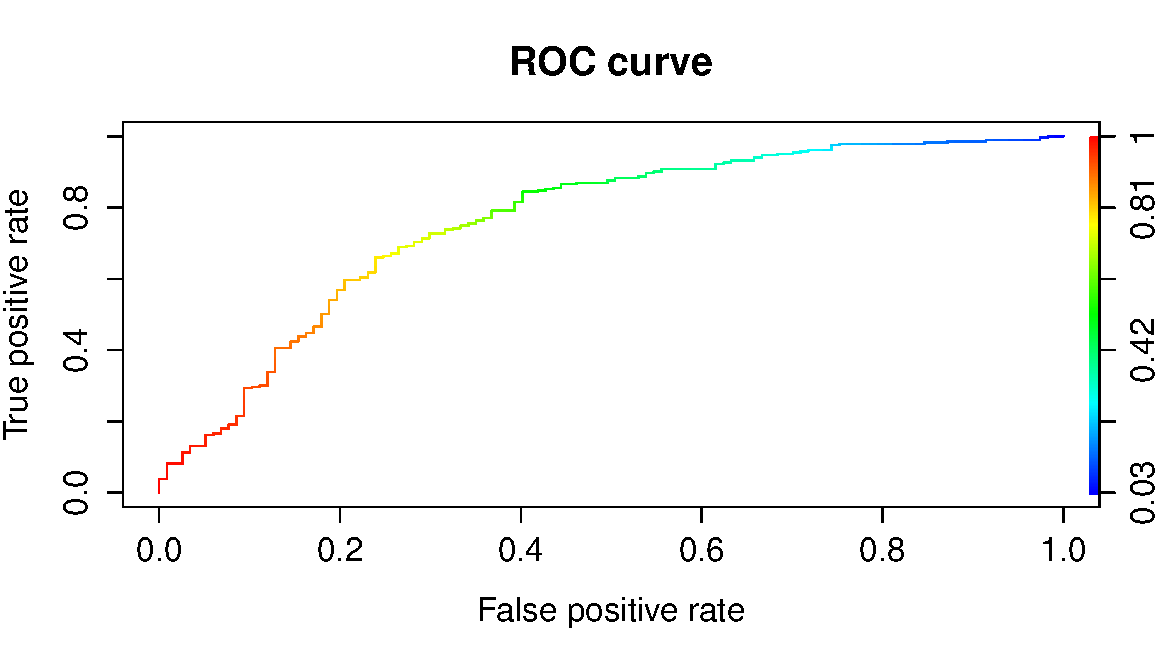
\includegraphics[width=0.98\textwidth]{ROCCurve.pdf}


\subsection*{Lift Curve}
\begin{Schunk}
\begin{Sinput}
> p.rocr.lift <- performance(p.rocr, "lift", "rpp")
> plot(p.rocr.lift, main="Lift Curve", colorize=T)
\end{Sinput}
\end{Schunk}
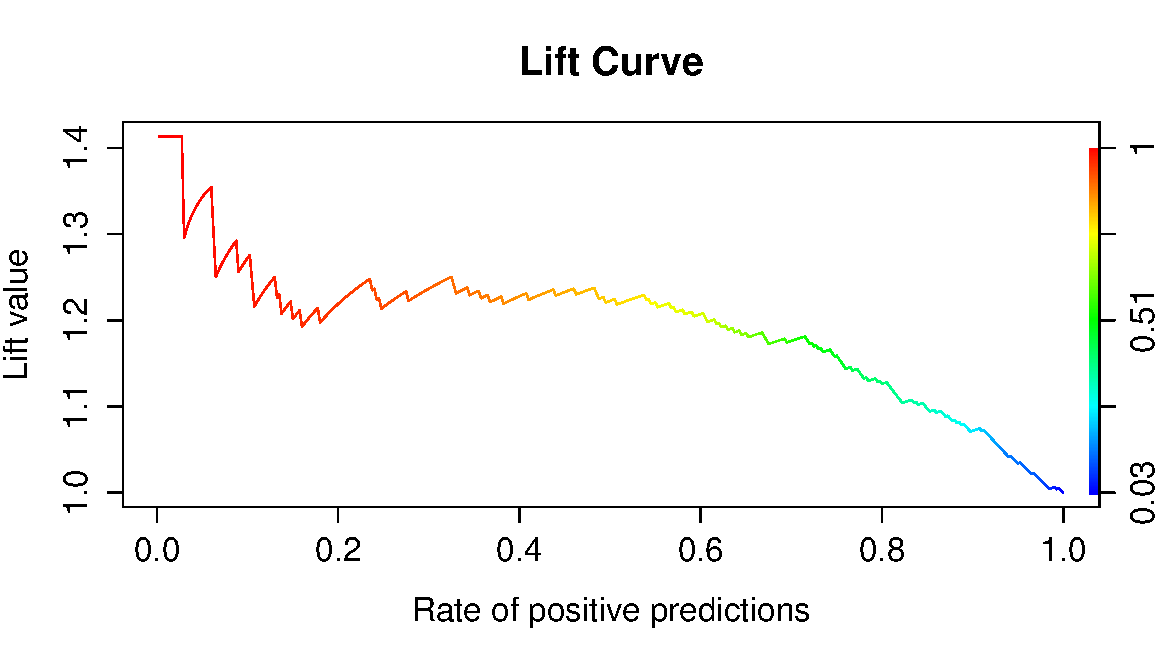
\includegraphics[width=0.98\textwidth]{LiftCurve.pdf}

\subsection{Classification Table with different cutoff values}
\begin{Schunk}
\begin{Sinput}
> calcNetProfit <- function(facts, preds, cutoff) {
+   vals <- sapply(preds, function(y) { ifelse(y<cutoff,0, 1) })  
+   ct <- CrossTable(facts, vals, dnn = c("Actual", "Predicted"))
+   print("Profit with cutoff")
+   print(cutoff)
+   profitFromCrossTable(ct)
+ }
> profitFromCrossTable <- function(ct) {
+   profit <- ct$t[1,1] * 100
+   loss <- ct$t[2,1] * -500
+   profit - loss
+ }
> s <- seq(0,1, by = .1)
> for(i in s) { print(calcNetProfit(gc.test$RESPONSE, p.test, i)) }
\end{Sinput}
\begin{Soutput}
   Cell Contents
|-------------------------|
|                       N |
|         N / Table Total |
|-------------------------|

 
Total Observations in Table:  400 

 
             | vals 
       facts |         1 | Row Total | 
-------------|-----------|-----------|
           0 |       117 |       117 | 
             |     0.292 |           | 
-------------|-----------|-----------|
           1 |       283 |       283 | 
             |     0.708 |           | 
-------------|-----------|-----------|
Column Total |       400 |       400 | 
-------------|-----------|-----------|

 
[1] "Profit with cutoff"
[1] 0
[1] 153200

 
   Cell Contents
|-------------------------|
|                       N |
| Chi-square contribution |
|           N / Row Total |
|           N / Col Total |
|         N / Table Total |
|-------------------------|

 
Total Observations in Table:  400 

 
             | Predicted 
      Actual |         0 |         1 | Row Total | 
-------------|-----------|-----------|-----------|
           0 |         6 |       111 |       117 | 
             |     7.630 |     0.136 |           | 
             |     0.051 |     0.949 |     0.292 | 
             |     0.857 |     0.282 |           | 
             |     0.015 |     0.278 |           | 
-------------|-----------|-----------|-----------|
           1 |         1 |       282 |       283 | 
             |     3.154 |     0.056 |           | 
             |     0.004 |     0.996 |     0.708 | 
             |     0.143 |     0.718 |           | 
             |     0.003 |     0.705 |           | 
-------------|-----------|-----------|-----------|
Column Total |         7 |       393 |       400 | 
             |     0.018 |     0.983 |           | 
-------------|-----------|-----------|-----------|

 
[1] "Profit with cutoff"
[1] 0.1
[1] 1100

 
   Cell Contents
|-------------------------|
|                       N |
| Chi-square contribution |
|           N / Row Total |
|           N / Col Total |
|         N / Table Total |
|-------------------------|

 
Total Observations in Table:  400 

 
             | Predicted 
      Actual |         0 |         1 | Row Total | 
-------------|-----------|-----------|-----------|
           0 |        21 |        96 |       117 | 
             |    25.620 |     1.708 |           | 
             |     0.179 |     0.821 |     0.292 | 
             |     0.840 |     0.256 |           | 
             |     0.052 |     0.240 |           | 
-------------|-----------|-----------|-----------|
           1 |         4 |       279 |       283 | 
             |    10.592 |     0.706 |           | 
             |     0.014 |     0.986 |     0.708 | 
             |     0.160 |     0.744 |           | 
             |     0.010 |     0.698 |           | 
-------------|-----------|-----------|-----------|
Column Total |        25 |       375 |       400 | 
             |     0.062 |     0.938 |           | 
-------------|-----------|-----------|-----------|

 
[1] "Profit with cutoff"
[1] 0.2
[1] 4100

 
   Cell Contents
|-------------------------|
|                       N |
| Chi-square contribution |
|           N / Row Total |
|           N / Col Total |
|         N / Table Total |
|-------------------------|

 
Total Observations in Table:  400 

 
             | Predicted 
      Actual |         0 |         1 | Row Total | 
-------------|-----------|-----------|-----------|
           0 |        38 |        79 |       117 | 
             |    29.847 |     4.758 |           | 
             |     0.325 |     0.675 |     0.292 | 
             |     0.691 |     0.229 |           | 
             |     0.095 |     0.198 |           | 
-------------|-----------|-----------|-----------|
           1 |        17 |       266 |       283 | 
             |    12.339 |     1.967 |           | 
             |     0.060 |     0.940 |     0.708 | 
             |     0.309 |     0.771 |           | 
             |     0.043 |     0.665 |           | 
-------------|-----------|-----------|-----------|
Column Total |        55 |       345 |       400 | 
             |     0.138 |     0.863 |           | 
-------------|-----------|-----------|-----------|

 
[1] "Profit with cutoff"
[1] 0.3
[1] 12300

 
   Cell Contents
|-------------------------|
|                       N |
| Chi-square contribution |
|           N / Row Total |
|           N / Col Total |
|         N / Table Total |
|-------------------------|

 
Total Observations in Table:  400 

 
             | Predicted 
      Actual |         0 |         1 | Row Total | 
-------------|-----------|-----------|-----------|
           0 |        49 |        68 |       117 | 
             |    28.007 |     7.002 |           | 
             |     0.419 |     0.581 |     0.292 | 
             |     0.613 |     0.212 |           | 
             |     0.122 |     0.170 |           | 
-------------|-----------|-----------|-----------|
           1 |        31 |       252 |       283 | 
             |    11.579 |     2.895 |           | 
             |     0.110 |     0.890 |     0.708 | 
             |     0.388 |     0.787 |           | 
             |     0.077 |     0.630 |           | 
-------------|-----------|-----------|-----------|
Column Total |        80 |       320 |       400 | 
             |     0.200 |     0.800 |           | 
-------------|-----------|-----------|-----------|

 
[1] "Profit with cutoff"
[1] 0.4
[1] 20400

 
   Cell Contents
|-------------------------|
|                       N |
| Chi-square contribution |
|           N / Row Total |
|           N / Col Total |
|         N / Table Total |
|-------------------------|

 
Total Observations in Table:  400 

 
             | Predicted 
      Actual |         0 |         1 | Row Total | 
-------------|-----------|-----------|-----------|
           0 |        62 |        55 |       117 | 
             |    35.660 |    12.046 |           | 
             |     0.530 |     0.470 |     0.292 | 
             |     0.614 |     0.184 |           | 
             |     0.155 |     0.138 |           | 
-------------|-----------|-----------|-----------|
           1 |        39 |       244 |       283 | 
             |    14.743 |     4.980 |           | 
             |     0.138 |     0.862 |     0.708 | 
             |     0.386 |     0.816 |           | 
             |     0.098 |     0.610 |           | 
-------------|-----------|-----------|-----------|
Column Total |       101 |       299 |       400 | 
             |     0.253 |     0.748 |           | 
-------------|-----------|-----------|-----------|

 
[1] "Profit with cutoff"
[1] 0.5
[1] 25700

 
   Cell Contents
|-------------------------|
|                       N |
| Chi-square contribution |
|           N / Row Total |
|           N / Col Total |
|         N / Table Total |
|-------------------------|

 
Total Observations in Table:  400 

 
             | Predicted 
      Actual |         0 |         1 | Row Total | 
-------------|-----------|-----------|-----------|
           0 |        75 |        42 |       117 | 
             |    31.938 |    16.270 |           | 
             |     0.641 |     0.359 |     0.292 | 
             |     0.556 |     0.158 |           | 
             |     0.188 |     0.105 |           | 
-------------|-----------|-----------|-----------|
           1 |        60 |       223 |       283 | 
             |    13.204 |     6.727 |           | 
             |     0.212 |     0.788 |     0.708 | 
             |     0.444 |     0.842 |           | 
             |     0.150 |     0.557 |           | 
-------------|-----------|-----------|-----------|
Column Total |       135 |       265 |       400 | 
             |     0.338 |     0.662 |           | 
-------------|-----------|-----------|-----------|

 
[1] "Profit with cutoff"
[1] 0.6
[1] 37500

 
   Cell Contents
|-------------------------|
|                       N |
| Chi-square contribution |
|           N / Row Total |
|           N / Col Total |
|         N / Table Total |
|-------------------------|

 
Total Observations in Table:  400 

 
             | Predicted 
      Actual |         0 |         1 | Row Total | 
-------------|-----------|-----------|-----------|
           0 |        83 |        34 |       117 | 
             |    27.379 |    18.444 |           | 
             |     0.709 |     0.291 |     0.292 | 
             |     0.516 |     0.142 |           | 
             |     0.207 |     0.085 |           | 
-------------|-----------|-----------|-----------|
           1 |        78 |       205 |       283 | 
             |    11.319 |     7.625 |           | 
             |     0.276 |     0.724 |     0.708 | 
             |     0.484 |     0.858 |           | 
             |     0.195 |     0.512 |           | 
-------------|-----------|-----------|-----------|
Column Total |       161 |       239 |       400 | 
             |     0.403 |     0.598 |           | 
-------------|-----------|-----------|-----------|

 
[1] "Profit with cutoff"
[1] 0.7
[1] 47300

 
   Cell Contents
|-------------------------|
|                       N |
| Chi-square contribution |
|           N / Row Total |
|           N / Col Total |
|         N / Table Total |
|-------------------------|

 
Total Observations in Table:  400 

 
             | Predicted 
      Actual |         0 |         1 | Row Total | 
-------------|-----------|-----------|-----------|
           0 |        90 |        27 |       117 | 
             |    19.936 |    18.588 |           | 
             |     0.769 |     0.231 |     0.292 | 
             |     0.466 |     0.130 |           | 
             |     0.225 |     0.068 |           | 
-------------|-----------|-----------|-----------|
           1 |       103 |       180 |       283 | 
             |     8.242 |     7.685 |           | 
             |     0.364 |     0.636 |     0.708 | 
             |     0.534 |     0.870 |           | 
             |     0.258 |     0.450 |           | 
-------------|-----------|-----------|-----------|
Column Total |       193 |       207 |       400 | 
             |     0.482 |     0.517 |           | 
-------------|-----------|-----------|-----------|

 
[1] "Profit with cutoff"
[1] 0.8
[1] 60500

 
   Cell Contents
|-------------------------|
|                       N |
| Chi-square contribution |
|           N / Row Total |
|           N / Col Total |
|         N / Table Total |
|-------------------------|

 
Total Observations in Table:  400 

 
             | Predicted 
      Actual |         0 |         1 | Row Total | 
-------------|-----------|-----------|-----------|
           0 |       103 |        14 |       117 | 
             |     7.516 |    15.433 |           | 
             |     0.880 |     0.120 |     0.292 | 
             |     0.383 |     0.107 |           | 
             |     0.258 |     0.035 |           | 
-------------|-----------|-----------|-----------|
           1 |       166 |       117 |       283 | 
             |     3.107 |     6.380 |           | 
             |     0.587 |     0.413 |     0.708 | 
             |     0.617 |     0.893 |           | 
             |     0.415 |     0.292 |           | 
-------------|-----------|-----------|-----------|
Column Total |       269 |       131 |       400 | 
             |     0.672 |     0.328 |           | 
-------------|-----------|-----------|-----------|

 
[1] "Profit with cutoff"
[1] 0.9
[1] 93300

 
   Cell Contents
|-------------------------|
|                       N |
|         N / Table Total |
|-------------------------|

 
Total Observations in Table:  400 

 
             | vals 
       facts |         0 | Row Total | 
-------------|-----------|-----------|
           0 |       117 |       117 | 
             |     0.292 |           | 
-------------|-----------|-----------|
           1 |       283 |       283 | 
             |     0.708 |           | 
-------------|-----------|-----------|
Column Total |       400 |       400 | 
-------------|-----------|-----------|

 
[1] "Profit with cutoff"
[1] 1
[1] 153200
\end{Soutput}
\end{Schunk}

\section*{Neural Network}
A Neural Network model is now fit to the train data. 

\begin{Schunk}
\begin{Sinput}
> library(nnet)
> nn <- nnet(RESPONSE ~ CHK_ACCT+DURATION+HISTORY+NEW_CAR+USED_CAR+FURNITURE+RADIO.TV+EDUCATION+RETRAINING+AMOUNT+SAV_ACCT+EMPLOYMENT+INSTALL_RATE+MALE_DIV+MALE_SINGLE+MALE_MAR_or_WID+CO.APPLICANT+GUARANTOR+PRESENT_RESIDENT+REAL_ESTATE+PROP_UNKN_NONE+AGE+OTHER_INSTALL+RENT+OWN_RES+NUM_CREDITS+JOB+NUM_DEPENDENTS+TELEPHONE+FOREIGN, size=20, data=gc.train, linout=FALSE, rang=.1, decay=5e-4, maxit=50)
\end{Sinput}
\begin{Soutput}
# weights:  901
initial  value 389.905872 
iter  10 value 369.026034
iter  20 value 368.813672
iter  30 value 359.861220
iter  40 value 335.341464
iter  50 value 276.665377
final  value 276.665377 
stopped after 50 iterations
\end{Soutput}
\begin{Sinput}
> nn
\end{Sinput}
\begin{Soutput}
a 43-20-1 network with 901 weights
inputs: CHK_ACCT1 CHK_ACCT2 CHK_ACCT3 DURATION HISTORY1 HISTORY2 HISTORY3 HISTORY4 NEW_CAR USED_CAR FURNITURE RADIO.TV EDUCATION RETRAINING AMOUNT SAV_ACCT1 SAV_ACCT2 SAV_ACCT3 SAV_ACCT4 EMPLOYMENT1 EMPLOYMENT2 EMPLOYMENT3 EMPLOYMENT4 INSTALL_RATE MALE_DIV MALE_SINGLE MALE_MAR_or_WID CO.APPLICANT GUARANTOR PRESENT_RESIDENT REAL_ESTATE PROP_UNKN_NONE AGE OTHER_INSTALL RENT OWN_RES NUM_CREDITS JOB1 JOB2 JOB3 NUM_DEPENDENTS TELEPHONE FOREIGN 
output(s): RESPONSE 
options were - entropy fitting  decay=5e-04
\end{Soutput}
\begin{Sinput}
> summary(nn)
\end{Sinput}
\begin{Soutput}
a 43-20-1 network with 901 weights
options were - entropy fitting  decay=5e-04
  b->h1  i1->h1  i2->h1  i3->h1  i4->h1  i5->h1  i6->h1  i7->h1  i8->h1  i9->h1 
   0.05    0.05    0.04   -0.08    0.04   -0.02   -0.08    0.07   -0.07    0.00 
i10->h1 i11->h1 i12->h1 i13->h1 i14->h1 i15->h1 i16->h1 i17->h1 i18->h1 i19->h1 
   0.03   -0.07    0.03    0.09    0.03   -0.08   -0.08    0.09    0.08   -0.07 
i20->h1 i21->h1 i22->h1 i23->h1 i24->h1 i25->h1 i26->h1 i27->h1 i28->h1 i29->h1 
   0.02   -0.05   -0.08   -0.03   -0.07    0.01    0.08    0.02    0.00    0.02 
i30->h1 i31->h1 i32->h1 i33->h1 i34->h1 i35->h1 i36->h1 i37->h1 i38->h1 i39->h1 
   0.06   -0.07   -0.09    0.02    0.04    0.03   -0.01    0.04   -0.01   -0.06 
i40->h1 i41->h1 i42->h1 i43->h1 
   0.07    0.05    0.04    0.02 
  b->h2  i1->h2  i2->h2  i3->h2  i4->h2  i5->h2  i6->h2  i7->h2  i8->h2  i9->h2 
  -0.07   -0.02    0.04   -0.01    0.04   -0.07   -0.04    0.08    0.06   -0.04 
i10->h2 i11->h2 i12->h2 i13->h2 i14->h2 i15->h2 i16->h2 i17->h2 i18->h2 i19->h2 
  -0.03   -0.07    0.08   -0.02    0.06    0.08    0.04   -0.03   -0.01   -0.05 
i20->h2 i21->h2 i22->h2 i23->h2 i24->h2 i25->h2 i26->h2 i27->h2 i28->h2 i29->h2 
   0.00   -0.06    0.00    0.06   -0.08    0.04    0.09    0.08    0.06   -0.03 
i30->h2 i31->h2 i32->h2 i33->h2 i34->h2 i35->h2 i36->h2 i37->h2 i38->h2 i39->h2 
   0.06   -0.06   -0.09    0.02    0.00    0.02    0.00    0.05   -0.06   -0.02 
i40->h2 i41->h2 i42->h2 i43->h2 
   0.04    0.02   -0.02   -0.05 
  b->h3  i1->h3  i2->h3  i3->h3  i4->h3  i5->h3  i6->h3  i7->h3  i8->h3  i9->h3 
   0.09    0.07    0.04   -0.02   -0.08    0.08   -0.03    0.00    0.09    0.05 
i10->h3 i11->h3 i12->h3 i13->h3 i14->h3 i15->h3 i16->h3 i17->h3 i18->h3 i19->h3 
   0.06    0.02   -0.04   -0.02   -0.09   -0.08   -0.04    0.07   -0.06   -0.01 
i20->h3 i21->h3 i22->h3 i23->h3 i24->h3 i25->h3 i26->h3 i27->h3 i28->h3 i29->h3 
  -0.02   -0.05   -0.02   -0.09   -0.02    0.07    0.05    0.07   -0.08    0.07 
i30->h3 i31->h3 i32->h3 i33->h3 i34->h3 i35->h3 i36->h3 i37->h3 i38->h3 i39->h3 
   0.04   -0.04   -0.06   -0.09    0.02   -0.02   -0.03    0.09    0.06    0.05 
i40->h3 i41->h3 i42->h3 i43->h3 
   0.06   -0.04    0.00   -0.03 
  b->h4  i1->h4  i2->h4  i3->h4  i4->h4  i5->h4  i6->h4  i7->h4  i8->h4  i9->h4 
   0.03    0.08   -0.04    0.05   -0.03   -0.06    0.06    0.04    0.00    0.06 
i10->h4 i11->h4 i12->h4 i13->h4 i14->h4 i15->h4 i16->h4 i17->h4 i18->h4 i19->h4 
   0.01   -0.02    0.00   -0.09    0.08    0.07   -0.06   -0.09    0.04    0.02 
i20->h4 i21->h4 i22->h4 i23->h4 i24->h4 i25->h4 i26->h4 i27->h4 i28->h4 i29->h4 
   0.09   -0.04    0.03   -0.04   -0.04    0.09    0.02    0.02    0.04   -0.07 
i30->h4 i31->h4 i32->h4 i33->h4 i34->h4 i35->h4 i36->h4 i37->h4 i38->h4 i39->h4 
  -0.07    0.01   -0.09    0.09    0.04    0.01   -0.07    0.04   -0.07    0.02 
i40->h4 i41->h4 i42->h4 i43->h4 
   0.00    0.06   -0.02    0.07 
  b->h5  i1->h5  i2->h5  i3->h5  i4->h5  i5->h5  i6->h5  i7->h5  i8->h5  i9->h5 
   0.03   -0.08    0.08   -0.07   -0.09   -0.05   -0.06   -0.01    0.05   -0.02 
i10->h5 i11->h5 i12->h5 i13->h5 i14->h5 i15->h5 i16->h5 i17->h5 i18->h5 i19->h5 
   0.05   -0.03    0.07    0.03    0.08    0.06    0.02    0.06    0.01    0.08 
i20->h5 i21->h5 i22->h5 i23->h5 i24->h5 i25->h5 i26->h5 i27->h5 i28->h5 i29->h5 
  -0.04    0.07    0.05   -0.07   -0.04    0.03    0.01    0.02   -0.09    0.01 
i30->h5 i31->h5 i32->h5 i33->h5 i34->h5 i35->h5 i36->h5 i37->h5 i38->h5 i39->h5 
   0.08   -0.01    0.04    0.07   -0.02   -0.05   -0.01   -0.06    0.09   -0.03 
i40->h5 i41->h5 i42->h5 i43->h5 
   0.04    0.00    0.09    0.07 
  b->h6  i1->h6  i2->h6  i3->h6  i4->h6  i5->h6  i6->h6  i7->h6  i8->h6  i9->h6 
  -0.04   -0.05   -0.03    0.03   -0.01    0.03    0.09    0.04   -0.07    0.03 
i10->h6 i11->h6 i12->h6 i13->h6 i14->h6 i15->h6 i16->h6 i17->h6 i18->h6 i19->h6 
  -0.07   -0.04    0.03    0.07    0.05   -0.06    0.02   -0.07    0.00    0.08 
i20->h6 i21->h6 i22->h6 i23->h6 i24->h6 i25->h6 i26->h6 i27->h6 i28->h6 i29->h6 
   0.00   -0.08   -0.02   -0.09   -0.04    0.00    0.08    0.08    0.03    0.08 
i30->h6 i31->h6 i32->h6 i33->h6 i34->h6 i35->h6 i36->h6 i37->h6 i38->h6 i39->h6 
   0.04   -0.01   -0.07   -0.06    0.03    0.03   -0.02    0.05   -0.03    0.02 
i40->h6 i41->h6 i42->h6 i43->h6 
   0.05    0.01    0.05    0.05 
  b->h7  i1->h7  i2->h7  i3->h7  i4->h7  i5->h7  i6->h7  i7->h7  i8->h7  i9->h7 
   1.08    1.37    0.11    0.24    4.57   -0.22    0.46   -0.95    1.41    0.91 
i10->h7 i11->h7 i12->h7 i13->h7 i14->h7 i15->h7 i16->h7 i17->h7 i18->h7 i19->h7 
   2.12   -1.44    0.26   -0.23   -0.34   -0.02   -0.04   -0.01    0.03   -0.39 
i20->h7 i21->h7 i22->h7 i23->h7 i24->h7 i25->h7 i26->h7 i27->h7 i28->h7 i29->h7 
  -0.32   -0.91    2.53   -0.15    1.04   -0.02    0.61    0.13   -0.05    0.16 
i30->h7 i31->h7 i32->h7 i33->h7 i34->h7 i35->h7 i36->h7 i37->h7 i38->h7 i39->h7 
   0.63    0.15   -1.64    1.80   -1.12    0.65    2.19    2.37    0.20    1.20 
i40->h7 i41->h7 i42->h7 i43->h7 
  -0.01    2.32   -2.07    0.13 
  b->h8  i1->h8  i2->h8  i3->h8  i4->h8  i5->h8  i6->h8  i7->h8  i8->h8  i9->h8 
   0.06    0.07   -0.04   -0.02    0.06   -0.01    0.07    0.05    0.08    0.06 
i10->h8 i11->h8 i12->h8 i13->h8 i14->h8 i15->h8 i16->h8 i17->h8 i18->h8 i19->h8 
   0.09   -0.05    0.01    0.01   -0.04   -0.06    0.04    0.03    0.07    0.00 
i20->h8 i21->h8 i22->h8 i23->h8 i24->h8 i25->h8 i26->h8 i27->h8 i28->h8 i29->h8 
  -0.03    0.06    0.09    0.02    0.00   -0.01    0.01    0.05    0.05   -0.02 
i30->h8 i31->h8 i32->h8 i33->h8 i34->h8 i35->h8 i36->h8 i37->h8 i38->h8 i39->h8 
   0.06    0.08   -0.03    0.09   -0.05    0.09    0.09    0.01   -0.07    0.09 
i40->h8 i41->h8 i42->h8 i43->h8 
   0.05   -0.08   -0.03    0.09 
  b->h9  i1->h9  i2->h9  i3->h9  i4->h9  i5->h9  i6->h9  i7->h9  i8->h9  i9->h9 
  -0.05   -0.04   -0.05   -0.02   -0.01    0.08    0.05   -0.04    0.06   -0.01 
i10->h9 i11->h9 i12->h9 i13->h9 i14->h9 i15->h9 i16->h9 i17->h9 i18->h9 i19->h9 
  -0.06   -0.02    0.01    0.00   -0.07    0.08   -0.08    0.05    0.08   -0.02 
i20->h9 i21->h9 i22->h9 i23->h9 i24->h9 i25->h9 i26->h9 i27->h9 i28->h9 i29->h9 
   0.07   -0.01    0.05   -0.02   -0.07    0.00    0.06    0.04    0.00    0.06 
i30->h9 i31->h9 i32->h9 i33->h9 i34->h9 i35->h9 i36->h9 i37->h9 i38->h9 i39->h9 
   0.04    0.06    0.07   -0.09   -0.06    0.08    0.09   -0.09    0.00   -0.07 
i40->h9 i41->h9 i42->h9 i43->h9 
   0.01   -0.06   -0.02    0.09 
  b->h10  i1->h10  i2->h10  i3->h10  i4->h10  i5->h10  i6->h10  i7->h10 
    0.02     0.01     0.06    -0.06     0.06    -0.07    -0.03     0.04 
 i8->h10  i9->h10 i10->h10 i11->h10 i12->h10 i13->h10 i14->h10 i15->h10 
    0.09     0.03    -0.07     0.05    -0.09    -0.05     0.06    -0.06 
i16->h10 i17->h10 i18->h10 i19->h10 i20->h10 i21->h10 i22->h10 i23->h10 
    0.07    -0.09    -0.04    -0.07     0.07     0.00     0.06     0.09 
i24->h10 i25->h10 i26->h10 i27->h10 i28->h10 i29->h10 i30->h10 i31->h10 
    0.00     0.04    -0.08    -0.08     0.08     0.08    -0.01     0.05 
i32->h10 i33->h10 i34->h10 i35->h10 i36->h10 i37->h10 i38->h10 i39->h10 
   -0.01     0.00     0.00    -0.06     0.04    -0.04    -0.09     0.02 
i40->h10 i41->h10 i42->h10 i43->h10 
   -0.03     0.02    -0.04    -0.01 
  b->h11  i1->h11  i2->h11  i3->h11  i4->h11  i5->h11  i6->h11  i7->h11 
   -0.05     0.04     0.02    -0.03    -0.03     0.09    -0.03    -0.03 
 i8->h11  i9->h11 i10->h11 i11->h11 i12->h11 i13->h11 i14->h11 i15->h11 
    0.01     0.07    -0.02     0.02    -0.03     0.06     0.04     0.09 
i16->h11 i17->h11 i18->h11 i19->h11 i20->h11 i21->h11 i22->h11 i23->h11 
   -0.03     0.00    -0.07     0.07    -0.03    -0.06    -0.03    -0.06 
i24->h11 i25->h11 i26->h11 i27->h11 i28->h11 i29->h11 i30->h11 i31->h11 
    0.09     0.03     0.05     0.01    -0.06    -0.02     0.08     0.07 
i32->h11 i33->h11 i34->h11 i35->h11 i36->h11 i37->h11 i38->h11 i39->h11 
   -0.08    -0.07    -0.07     0.01     0.01     0.03    -0.08    -0.01 
i40->h11 i41->h11 i42->h11 i43->h11 
   -0.02     0.03     0.05    -0.04 
  b->h12  i1->h12  i2->h12  i3->h12  i4->h12  i5->h12  i6->h12  i7->h12 
    0.04     0.03    -0.02    -0.09     0.04    -0.05    -0.08     0.00 
 i8->h12  i9->h12 i10->h12 i11->h12 i12->h12 i13->h12 i14->h12 i15->h12 
   -0.03    -0.05    -0.07     0.02    -0.07     0.06    -0.08     1.42 
i16->h12 i17->h12 i18->h12 i19->h12 i20->h12 i21->h12 i22->h12 i23->h12 
    0.01     0.06    -0.10     0.05     0.06    -0.05    -0.01     0.07 
i24->h12 i25->h12 i26->h12 i27->h12 i28->h12 i29->h12 i30->h12 i31->h12 
   -0.02    -0.09     0.00     0.06     0.04     0.01     0.00     0.02 
i32->h12 i33->h12 i34->h12 i35->h12 i36->h12 i37->h12 i38->h12 i39->h12 
   -0.02    -0.61     0.00    -0.05     0.06    -0.04    -0.03     0.03 
i40->h12 i41->h12 i42->h12 i43->h12 
   -0.05    -0.09    -0.07    -0.02 
  b->h13  i1->h13  i2->h13  i3->h13  i4->h13  i5->h13  i6->h13  i7->h13 
    0.01    -0.06     0.07     0.00    -0.02    -0.01    -0.06    -0.09 
 i8->h13  i9->h13 i10->h13 i11->h13 i12->h13 i13->h13 i14->h13 i15->h13 
    0.05    -0.04    -0.05     0.00    -0.06     0.04     0.02     0.11 
i16->h13 i17->h13 i18->h13 i19->h13 i20->h13 i21->h13 i22->h13 i23->h13 
    0.07    -0.08     0.04     0.02     0.06     0.09    -0.05     0.07 
i24->h13 i25->h13 i26->h13 i27->h13 i28->h13 i29->h13 i30->h13 i31->h13 
    0.03     0.06     0.08    -0.08    -0.03    -0.09     0.01    -0.06 
i32->h13 i33->h13 i34->h13 i35->h13 i36->h13 i37->h13 i38->h13 i39->h13 
    0.06    -0.04     0.00    -0.02     0.08    -0.06     0.08    -0.01 
i40->h13 i41->h13 i42->h13 i43->h13 
    0.02     0.00    -0.04    -0.09 
  b->h14  i1->h14  i2->h14  i3->h14  i4->h14  i5->h14  i6->h14  i7->h14 
   -0.05    -0.06    -0.06    -0.05    -0.03     0.08    -0.03    -0.07 
 i8->h14  i9->h14 i10->h14 i11->h14 i12->h14 i13->h14 i14->h14 i15->h14 
   -0.03     0.02     0.01     0.03     0.02    -0.07     0.04    -0.08 
i16->h14 i17->h14 i18->h14 i19->h14 i20->h14 i21->h14 i22->h14 i23->h14 
   -0.08     0.03     0.03     0.06    -0.08    -0.05    -0.04    -0.09 
i24->h14 i25->h14 i26->h14 i27->h14 i28->h14 i29->h14 i30->h14 i31->h14 
    0.06    -0.03     0.05     0.03    -0.04     0.09     0.05    -0.02 
i32->h14 i33->h14 i34->h14 i35->h14 i36->h14 i37->h14 i38->h14 i39->h14 
   -0.09    -0.05    -0.04     0.07    -0.03     0.07    -0.01     0.02 
i40->h14 i41->h14 i42->h14 i43->h14 
   -0.01     0.09    -0.06    -0.07 
  b->h15  i1->h15  i2->h15  i3->h15  i4->h15  i5->h15  i6->h15  i7->h15 
    0.01     0.08    -0.08    -0.01    -0.05    -0.06    -0.09     0.08 
 i8->h15  i9->h15 i10->h15 i11->h15 i12->h15 i13->h15 i14->h15 i15->h15 
    0.08    -0.03    -0.02     0.06    -0.03     0.06     0.07    -0.07 
i16->h15 i17->h15 i18->h15 i19->h15 i20->h15 i21->h15 i22->h15 i23->h15 
   -0.02    -0.08     0.04    -0.06     0.08    -0.01     0.05     0.03 
i24->h15 i25->h15 i26->h15 i27->h15 i28->h15 i29->h15 i30->h15 i31->h15 
   -0.04    -0.07     0.09    -0.07    -0.03     0.08    -0.03    -0.03 
i32->h15 i33->h15 i34->h15 i35->h15 i36->h15 i37->h15 i38->h15 i39->h15 
   -0.09     0.08     0.09     0.06    -0.02    -0.01     0.05     0.08 
i40->h15 i41->h15 i42->h15 i43->h15 
    0.03    -0.03     0.02     0.02 
  b->h16  i1->h16  i2->h16  i3->h16  i4->h16  i5->h16  i6->h16  i7->h16 
   -0.02     0.02     0.07    -0.02    -0.06     0.04     0.01    -0.01 
 i8->h16  i9->h16 i10->h16 i11->h16 i12->h16 i13->h16 i14->h16 i15->h16 
   -0.03     0.08     0.00     0.08     0.01     0.02     0.00    -0.05 
i16->h16 i17->h16 i18->h16 i19->h16 i20->h16 i21->h16 i22->h16 i23->h16 
   -0.01     0.09    -0.06    -0.05     0.09     0.02     0.08     0.04 
i24->h16 i25->h16 i26->h16 i27->h16 i28->h16 i29->h16 i30->h16 i31->h16 
    0.09    -0.07    -0.07     0.00     0.03    -0.09     0.09     0.06 
i32->h16 i33->h16 i34->h16 i35->h16 i36->h16 i37->h16 i38->h16 i39->h16 
   -0.05    -0.07     0.02    -0.03    -0.01     0.05    -0.07    -0.07 
i40->h16 i41->h16 i42->h16 i43->h16 
   -0.04     0.03     0.07    -0.01 
  b->h17  i1->h17  i2->h17  i3->h17  i4->h17  i5->h17  i6->h17  i7->h17 
    0.07     0.09    -0.07     0.03    -0.02    -0.05     0.01    -0.04 
 i8->h17  i9->h17 i10->h17 i11->h17 i12->h17 i13->h17 i14->h17 i15->h17 
    0.09    -0.08    -0.03    -0.08     0.06    -0.03     0.08    -0.04 
i16->h17 i17->h17 i18->h17 i19->h17 i20->h17 i21->h17 i22->h17 i23->h17 
    0.01    -0.03    -0.06     0.07     0.06     0.09     0.08    -0.04 
i24->h17 i25->h17 i26->h17 i27->h17 i28->h17 i29->h17 i30->h17 i31->h17 
   -0.06     0.06     0.08    -0.04     0.07    -0.07     0.05    -0.08 
i32->h17 i33->h17 i34->h17 i35->h17 i36->h17 i37->h17 i38->h17 i39->h17 
   -0.02     0.00     0.00     0.07    -0.08     0.07     0.04     0.08 
i40->h17 i41->h17 i42->h17 i43->h17 
   -0.04    -0.07    -0.01     0.06 
  b->h18  i1->h18  i2->h18  i3->h18  i4->h18  i5->h18  i6->h18  i7->h18 
   -0.08    -0.09    -0.04    -0.05     0.08     0.02    -0.01    -0.01 
 i8->h18  i9->h18 i10->h18 i11->h18 i12->h18 i13->h18 i14->h18 i15->h18 
   -0.03     0.05     0.09    -0.04     0.02     0.03     0.09     0.09 
i16->h18 i17->h18 i18->h18 i19->h18 i20->h18 i21->h18 i22->h18 i23->h18 
   -0.05     0.08    -0.04    -0.01     0.09    -0.06     0.02     0.03 
i24->h18 i25->h18 i26->h18 i27->h18 i28->h18 i29->h18 i30->h18 i31->h18 
    0.04    -0.03     0.01     0.08    -0.04    -0.02     0.00    -0.02 
i32->h18 i33->h18 i34->h18 i35->h18 i36->h18 i37->h18 i38->h18 i39->h18 
   -0.06     0.00    -0.05    -0.02     0.00     0.00    -0.02    -0.05 
i40->h18 i41->h18 i42->h18 i43->h18 
    0.08     0.05    -0.01    -0.08 
  b->h19  i1->h19  i2->h19  i3->h19  i4->h19  i5->h19  i6->h19  i7->h19 
    0.01    -0.06    -0.03    -0.09    -0.05    -0.04    -0.03     0.04 
 i8->h19  i9->h19 i10->h19 i11->h19 i12->h19 i13->h19 i14->h19 i15->h19 
    0.05     0.02     0.05     0.09     0.06    -0.02    -0.03     0.09 
i16->h19 i17->h19 i18->h19 i19->h19 i20->h19 i21->h19 i22->h19 i23->h19 
   -0.02    -0.01    -0.04    -0.06     0.06    -0.07     0.01     0.03 
i24->h19 i25->h19 i26->h19 i27->h19 i28->h19 i29->h19 i30->h19 i31->h19 
   -0.04    -0.02     0.08    -0.03    -0.01     0.04     0.08    -0.03 
i32->h19 i33->h19 i34->h19 i35->h19 i36->h19 i37->h19 i38->h19 i39->h19 
   -0.06     0.02     0.02     0.05     0.03    -0.05     0.05    -0.09 
i40->h19 i41->h19 i42->h19 i43->h19 
    0.07     0.02     0.05     0.05 
  b->h20  i1->h20  i2->h20  i3->h20  i4->h20  i5->h20  i6->h20  i7->h20 
    1.35     3.90    -1.78   -20.81     1.22     7.35    -0.16     1.65 
 i8->h20  i9->h20 i10->h20 i11->h20 i12->h20 i13->h20 i14->h20 i15->h20 
   -8.87    11.30    -2.86     3.77    -5.79     2.40    -2.28     0.00 
i16->h20 i17->h20 i18->h20 i19->h20 i20->h20 i21->h20 i22->h20 i23->h20 
    0.64    -6.01    -5.06    -6.76     8.92    -4.95    -6.09     1.91 
i24->h20 i25->h20 i26->h20 i27->h20 i28->h20 i29->h20 i30->h20 i31->h20 
    6.81     6.63    -6.70    -4.85     4.49    -2.51    -1.12     0.73 
i32->h20 i33->h20 i34->h20 i35->h20 i36->h20 i37->h20 i38->h20 i39->h20 
    8.43    -0.98    -2.59    -0.98    -5.54    -1.58     4.69     5.23 
i40->h20 i41->h20 i42->h20 i43->h20 
   -7.73     3.74   -13.14    -4.54 
  b->o  h1->o  h2->o  h3->o  h4->o  h5->o  h6->o  h7->o  h8->o  h9->o h10->o 
 -0.13  -0.06  -0.16   0.05  -0.22  -0.12  -0.04   4.50  -0.01  -0.22   0.02 
h11->o h12->o h13->o h14->o h15->o h16->o h17->o h18->o h19->o h20->o 
 -0.26  -0.47  -0.15   0.09   0.04   0.08   0.13  -0.28  -0.15  -2.76 
\end{Soutput}
\end{Schunk}

\subsection*{Using the model with the test data}
The test data is then run through the model
\begin{Schunk}
\begin{Sinput}
> nn.pred <- predict(nn, gc.test, type="raw")
> summary(nn.pred)
\end{Sinput}
\begin{Soutput}
       V1          
 Min.   :0.007196  
 1st Qu.:0.394270  
 Median :0.911725  
 Mean   :0.711669  
 3rd Qu.:0.911725  
 Max.   :0.911726  
\end{Soutput}
\end{Schunk}

\subsection*{ROC Curve}
\begin{Schunk}
\begin{Sinput}
> library(ROCR)
> nn.rocr <- prediction(nn.pred, gc.test$RESPONSE)
> nn.rocr.roc <- performance(nn.rocr, "tpr", "fpr")
> plot(nn.rocr.roc, main="ROC Curve", colorize=T)
\end{Sinput}
\end{Schunk}
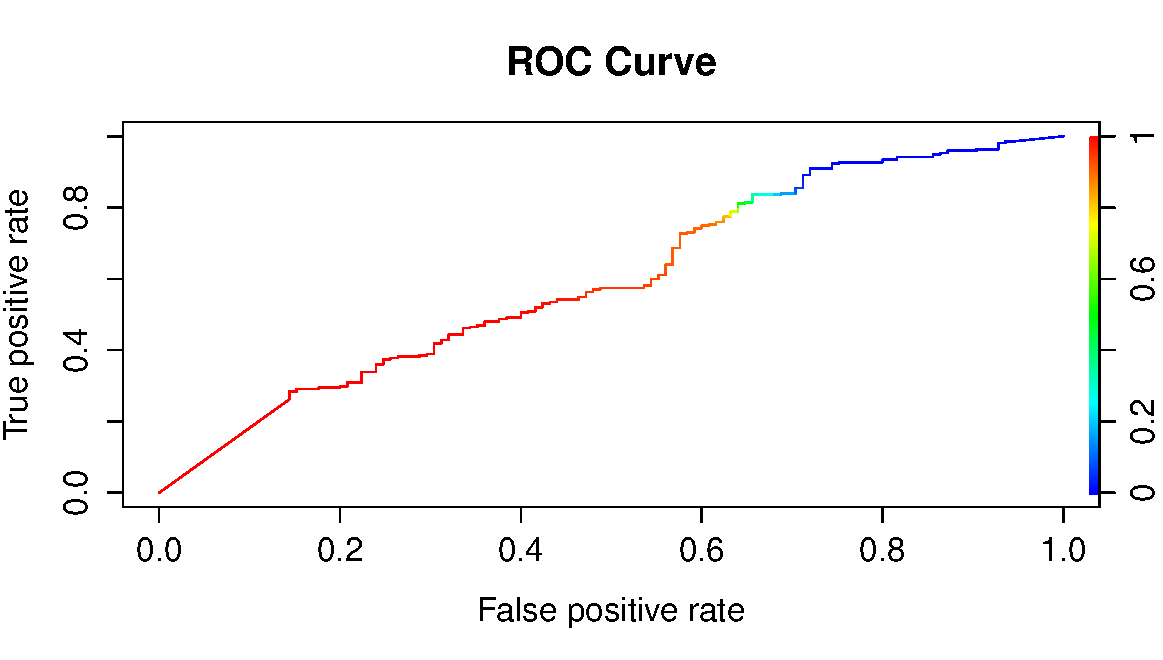
\includegraphics[width=0.98\textwidth]{ROCCurveNN.pdf}


\subsection*{Lift Curve}
\begin{Schunk}
\begin{Sinput}
> nn.rocr.lift <- performance(nn.rocr, "lift", "rpp")
> plot(nn.rocr.lift, main="Lift Curve", colorize=T)
\end{Sinput}
\end{Schunk}
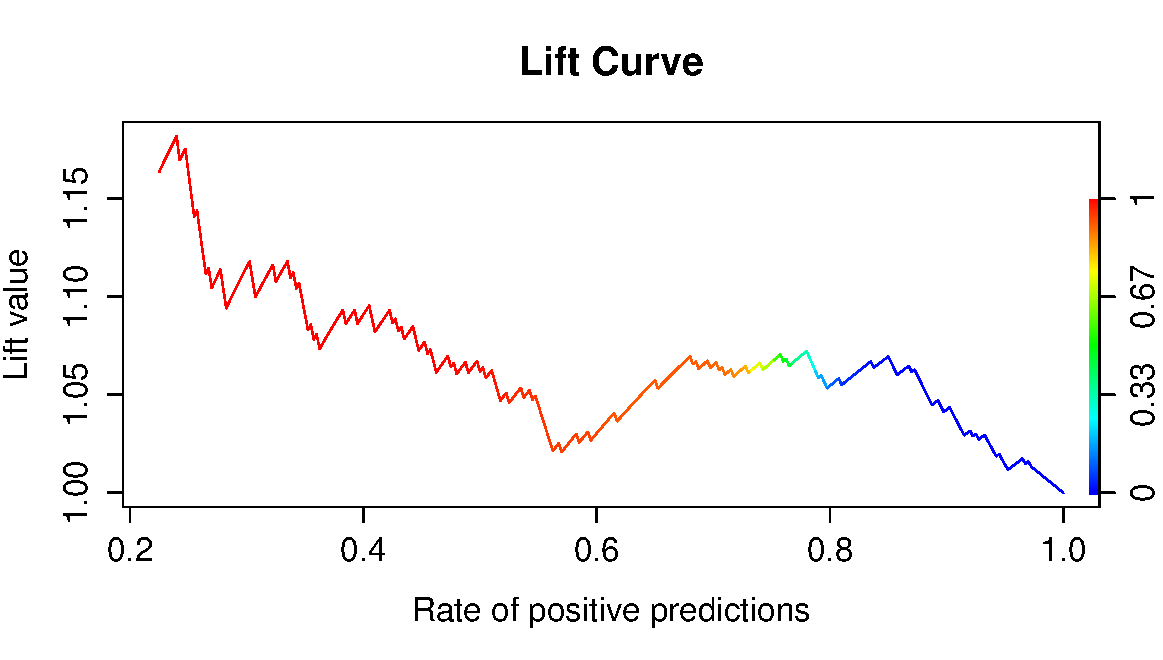
\includegraphics[width=0.98\textwidth]{LiftCurveNN.pdf}


\section*{Lesson 3 Question and Answer}
\subsection*1\emph{Comments on the models}
\\
\\
\noindent
I had trouble getting a good fit using a Neural Network. I think the sample size of the data is not sufficiently large to train the network in a more significant way than with the Logistical Regression model. NN is noticibly slower. I generated ROC and Lift Curves for both approaches and Logistical Regression clearly out performs NN for the given data. I think this is a function of the size of the sample though.
\newline
\newline
\noindent
I feel NN may outperform Logistical Regression when there may be many predictors with more complex relationships than presently given and the sample train data is sufficiently large. 
With Neural Networks it is not easy to say what the model is doing and why, and there are no statistical confidence indicators like Degrees of Freedom, etc.  


\subsection*2\emph{If you want to select 275 customers from the validation data set, which model would you adopt for credit rating? Why?}
\newline
\newline
\noindent
I would choose the Logistical Regression model as it clearly shows a greater Lift, and is explainable using statistical methods. It also handles categorical data in a more understandable way. 
\newline
\newline
\noindent
More specifically, I would use the Logistical Regression model with a high cutoff value, > 90\% approximately. 
\newline
\newline
\noindent
I should note, I played for hours with NN to get a good fit, and was never completely satisfied. I don't think NN is inferior to Logistical Regression, just not as suited to the current data. 

\end{document}
